\documentclass{article}

\usepackage{fancyhdr}
\usepackage{extramarks}
\usepackage{amsmath}
\usepackage{amsthm}
\usepackage{amsfonts}
\usepackage{tikz}
\usepackage{tikz-qtree}
\usepackage[plain]{algorithm}
\usepackage{algpseudocode}
\usepackage{listings}
\usepackage{enumerate}
\lstset{breaklines=true}

\usetikzlibrary{automata,positioning,calc}

%
% Basic Document Settings
%

\topmargin=-0.45in
\evensidemargin=0in
\oddsidemargin=0in
\textwidth=6.5in
\textheight=9.0in
\headsep=0.25in

\linespread{1.1}

\pagestyle{fancy}
\lhead{\hmwkAuthorName}
\chead{\hmwkClass\ (\hmwkClassInstructor): \hmwkTitle}
\rhead{\firstxmark}
\lfoot{\lastxmark}
\cfoot{\thepage}

\renewcommand\headrulewidth{0.4pt}
\renewcommand\footrulewidth{0.4pt}

\setlength\parindent{0pt}

%
% Create Problem Sections
%

\newcommand{\enterProblemHeader}[1]{
    \nobreak\extramarks{}{Problem \arabic{#1} continued on next page\ldots}\nobreak{}
    \nobreak\extramarks{Problem \arabic{#1} (continued)}{Problem \arabic{#1} continued on next page\ldots}\nobreak{}
}

\newcommand{\exitProblemHeader}[1]{
    \nobreak\extramarks{Problem \arabic{#1} (continued)}{Problem \arabic{#1} continued on next page\ldots}\nobreak{}
    \stepcounter{#1}
    \nobreak\extramarks{Problem \arabic{#1}}{}\nobreak{}
}

\newcommand{\bipgraph}[2]{%
    \begin{tikzpicture}[every node/.style={circle,draw}]
    \foreach \xitem in {1,...,#1}
    {%
    % first set
    \node at (0,\xitem) (a\xitem) {};
    % second set
    \node at (2,\xitem) (b\xitem) {};   
    }%

    % connections
    \foreach \x [count=\xi] in {#2}
    {% 
    \foreach \tritem in \x % <-- Here no braces to make it a foreach list also not \xi but \x
    \draw(a\xi) -- (b\tritem);
    }
    \end{tikzpicture}  
}

\newcommand{\bipgraphComplete}[1]{%
    \begin{tikzpicture}[every node/.style={circle,draw}]
    \foreach \xitem in {1,...,#1}
    {%
    % first set
    \node at (0,\xitem) (a\xitem) {};
    % second set
    \node at (2,\xitem) (b\xitem) {};   
    }%

    % connections
    \foreach \x in {1,...,#1}
    {% 
    \foreach \y in {1,...,#1}
        \draw(a\x) -- (b\y);
    }
    \end{tikzpicture}  
}

\setcounter{secnumdepth}{0}
\newcounter{partCounter}
\newcounter{homeworkProblemCounter}
\setcounter{homeworkProblemCounter}{1}
\nobreak\extramarks{Problem \arabic{homeworkProblemCounter}}{}\nobreak{}

%
% Homework Problem Environment
%
% This environment takes an optional argument. When given, it will adjust the
% problem counter. This is useful for when the problems given for your
% assignment aren't sequential. See the last 3 problems of this template for an
% example.
%
\newenvironment{homeworkProblem}[1][-1]{
    \ifnum#1>0
        \setcounter{homeworkProblemCounter}{#1}
    \fi
    \section{Problem \arabic{homeworkProblemCounter}}
    \setcounter{partCounter}{1}
    \enterProblemHeader{homeworkProblemCounter}
}{
    \exitProblemHeader{homeworkProblemCounter}
}

%
% Homework Details
%   - Title
%   - Due date
%   - Class
%   - Section/Time
%   - Instructor
%   - Author
%

\newcommand{\hmwkTitle}{Homework\ \#7}
\newcommand{\hmwkDueDate}{February 18, 2015}
\newcommand{\hmwkClass}{Graph Theory}
\newcommand{\hmwkClassTime}{MWF 9:15}
\newcommand{\hmwkClassInstructor}{Professor McGinley}
\newcommand{\hmwkAuthorName}{Rick Sullivan}

%
% Title Page
%

\title{
    \vspace{2in}
    \textmd{\textbf{\hmwkClass:\ \hmwkTitle}}\\
    \normalsize\vspace{0.1in}\small{Due\ on\ \hmwkDueDate}\\
    \vspace{0.1in}\large{\textit{\hmwkClassInstructor\ \hmwkClassTime}}
    \vspace{3in}
}

\author{\textbf{\hmwkAuthorName}}
\date{}

\renewcommand{\part}[1]{\textbf{\large Part \Alph{partCounter}}\stepcounter{partCounter}\\}

%
% Various Helper Commands
%

% Useful for algorithms
\newcommand{\alg}[1]{\textsc{\bfseries \footnotesize #1}}

% For derivatives
\newcommand{\deriv}[1]{\frac{\mathrm{d}}{\mathrm{d}x} (#1)}

% For partial derivatives
\newcommand{\pderiv}[2]{\frac{\partial}{\partial #1} (#2)}

% Integral dx
\newcommand{\dx}{\mathrm{d}x}

% Alias for the Solution section header
\newcommand{\solution}{\textbf{\large Solution}}

% Probability commands: Expectation, Variance, Covariance, Bias
\newcommand{\E}{\mathrm{E}}
\newcommand{\Var}{\mathrm{Var}}
\newcommand{\Cov}{\mathrm{Cov}}
\newcommand{\Bias}{\mathrm{Bias}}

\begin{document}

\maketitle

\pagebreak

\begin{homeworkProblem}
	Find the maximum matching of \(G\). Prove that it is maximum by giving the minimum vertex cover, of the same size as the matching.
\\

	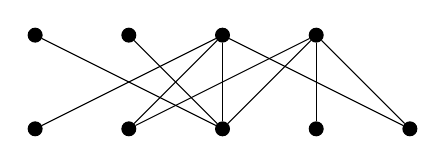
\begin{tikzpicture}[vertex/.style={circle,draw,fill=black,inner sep=0pt,minimum size=5pt}]
		\node[vertex] (a) {};
		\node[vertex] (b) [right=1cm of a] {};
		\node[vertex] (c) [right=1cm of b] {};
		\node[vertex] (d) [right=1cm of c] {};
		\node[vertex] (e) [below=1cm of a] {};
		\node[vertex] (f) [right=1cm of e] {};
		\node[vertex] (g) [right=1cm of f] {};
		\node[vertex] (h) [right=1cm of g] {};
		\node[vertex] (i) [right=1cm of h] {};

		\draw (a) -- (g);
		\draw (b) -- (g);
		\draw (c) -- (e);
		\draw (c) -- (f);
		\draw (c) -- (g);
		\draw (c) -- (i);
		\draw (d) -- (f);
		\draw (d) -- (g);
		\draw (d) -- (h);
		\draw (d) -- (i);
	\end{tikzpicture}


	\textbf{Solution}
	\\

	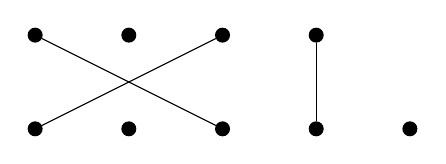
\begin{tikzpicture}[vertex/.style={circle,draw,fill=black,inner sep=0pt,minimum size=5pt}]
		\node[vertex] (a) {};
		\node[vertex] (b) [right=1cm of a] {};
		\node[vertex] (c) [right=1cm of b] {};
		\node[vertex] (d) [right=1cm of c] {};
		\node[vertex] (e) [below=1cm of a] {};
		\node[vertex] (f) [right=1cm of e] {};
		\node[vertex] (g) [right=1cm of f] {};
		\node[vertex] (h) [right=1cm of g] {};
		\node[vertex] (i) [right=1cm of h] {};

		\draw (a) -- (g);
		\draw (c) -- (e);
		\draw (d) -- (h);
	\end{tikzpicture}
	\\

	The minimum vertex cover consists of three vertices, either the top or bottom set of three non-isolated vertices.
	This is the same size as the matching given.
\end{homeworkProblem}
\begin{homeworkProblem}
	Determine the number of perfect matchings in \(K_{p,p}\).
\\

	\textbf{Solution}
\\
	\bipgraphComplete{2}
	\bipgraphComplete{3}
	\bipgraphComplete{4}
	\bipgraphComplete{5}
\\
	In all complete bipartite graphs, we can connect any vertex in one set to any vertex in the opposite set. When choosing a perfect matching, we have \(p\) choices for matching the first vertex, followed by \(p-1\) for the next, and so on. Therefore, we have \(p!\) perfect matchings.
\end{homeworkProblem}
\begin{homeworkProblem}
	Determine the number of perfect matchings in \(K_{2p}\).
\\

	\textbf{Solution}
\\

	In constructing the perfect matching, we first have \(2p-1\) choices to match any given vertex. The next vertex then has \(2p-3\) choices to match with, and so on. In this manner, we can consider matching \(p\) of the vertices to another, with \((2p-1)*(2p-3)*...*(3)*(1)\) choices. There will be \(p\) elements with choices given in the manner \[\prod_{i=1}^p2p-2i+1\]
Which gives the total number of perfect matchings.
\end{homeworkProblem}
\begin{homeworkProblem}
	Show that a tree has at most one perfect matching.
\\

	\textbf{Solution}
\\
\begin{proof}
	If the tree has an odd number of vertices, it cannot have a perfect matching.
\\

	Consider a tree with an even number of vertices.
\\

	Base case: \(n=2\). The tree has one perfect matching on the single edge.
\\

	Inductive case: Assume a tree \(T\) has one or zero perfect matchings. 
If \(T\) has zero perfect matchings, adding one vertex to \(T\) can add at most one perfect matching, as it can only connect to a single vertex.
If \(T\) has one matching, adding a vertex means that \(T\) has an odd number of vertices, so it has no perfect matchings.
\\

	Therefore, any tree will have at most one perfect matching.
\end{proof}
\end{homeworkProblem}
\end{document}
